%% LaTeX-Beamer template for KIT design
%% by Erik Burger, Christian Hammer
%% title picture by Klaus Krogmann
%%
%% version 2.1
%%
%% mostly compatible to KIT corporate design v2.0
%% http://intranet.kit.edu/gestaltungsrichtlinien.php
%%
%% Problems, bugs and comments to
%% burger@kit.edu

\documentclass[18pt]{beamer}

%% SLIDE FORMAT

% use 'beamerthemekit' for standard 4:3 ratio
% for widescreen slides (16:9), use 'beamerthemekitwide'

\usepackage{templates/beamerthemekit}
% \usepackage{templates/beamerthemekitwide}

\usepackage[utf8]{inputenc}
\usepackage{hyperref}
\usepackage{listings}
\usepackage{color}
\usepackage{xcolor}
\usepackage{colortbl}
\usepackage{array}
%\usepackage{tikz}
%\usetikzlibrary{calc,shapes.multipart,chains,arrows}
\usepackage{amsmath}
\usepackage{amssymb}
\usepackage{mathrsfs}
\usepackage{eurosym}

\definecolor{lime}{HTML}{8FFF53}
\definecolor{darkgrey}{HTML}{5A5A5A}
\definecolor{awesome}{HTML}{FF2252}
\definecolor{lightgreen}{HTML}{E0FF98}

\newcommand{\quotes}[1]{``#1''}

%% TITLE PICTURE

% if a custom picture is to be used on the title page, copy it into the 'logos'
% directory, in the line below, replace 'mypicture' with the
% filename (without extension) and uncomment the following line
% (picture proportions: 63 : 20 for standard, 169 : 40 for wide
% *.eps format if you use latex+dvips+ps2pdf,
% *.jpg/*.png/*.pdf if you use pdflatex)

\titleimage{greendrop}

%% TITLE LOGO

% for a custom logo on the front page, copy your file into the 'logos'
% directory, insert the filename in the line below and uncomment it

%\titlelogo{mylogo}

% (*.eps format if you use latex+dvips+ps2pdf,
% *.jpg/*.png/*.pdf if you use pdflatex)

%% TikZ INTEGRATION

% use these packages for PCM symbols and UML classes
% \usepackage{templates/tikzkit}
% \usepackage{templates/tikzuml}

% the presentation starts here

\title[Ganz viele Tipps und dann noch Debugging]{Programmieren:\\ Ganz viele Tipps und dann noch Debugging}
\subtitle{Tutorium 30}
\author{YouniS Bensalah}
\date{January 29, 2016}

\institute{Chair for Software Design and Quality}

% Bibliography

\usepackage[citestyle=authoryear,bibstyle=numeric,hyperref,backend=biber]{biblatex}
\addbibresource{templates/example.bib}
\bibhang1em

\begin{document}

% change the following line to "ngerman" for German style date and logos
\selectlanguage{english}

%title page
\begin{frame}
\titlepage
\end{frame}

%table of contents
\begin{frame}{Heute}
\tableofcontents
\end{frame}

\section{Organisatorisches}

\begin{frame}{Organisatorisches}
    \begin{itemize}
        \item Die Tutorien finden bis enschließlich \textbf{09.12.2016} statt.
        \item Die Anmeldung für den Übungsschein über das \textbf{Campus Management Portal} sollte jetzt wieder laufen.
    \end{itemize}
    \begin{alertblock}{Wichtig}
        \begin{itemize}
            \item Aufgrund eines technischen Problems bei allen Anmeldungen vor dem \textbf{27.01.2016} müssen alle Studenten,
            die sich vor diesem Datum angemeldet haben, sich im System ab- und erneut wieder anmelden.
            \item Die Anmeldung ist nur nach erfolgreicher Ab- und Anmeldung gültig.
            \item Exportieren Sie bitte nach der Anmeldung die Liste aller angemeldeten Prüfungen als PDF
            und bewahren Sie diese bis Ende der Bearbeitungszeit der Abschlussaufgaben auf.
        \end{itemize}
    \end{alertblock}
\end{frame}

\section{Ganz viele Tipps}

\begin{frame}{\quad}
    \center
    \Huge{Ganz viele Tipps \dots}
\end{frame}

\begin{frame}{\quad}
    \center
    \Huge{\textbf{1}}
\end{frame}

\begin{frame}{Tipp 1}
    \begin{block}{}
        \center
        \textsc{\quotes{Think first, code later.\\ Programming is not the act of writing code.}}
    \end{block}
\end{frame}

\begin{frame}{Tipp 1: Think first, code later.}
    \begin{itemize}
        \item Es geht vielmehr darum, Lösungen zu finden.
        \item Man sollte einen genauen Plan haben, bevor man anfängt irgendwelchen Code zu schreiben.
    \end{itemize}
\end{frame}

\begin{frame}{Tipp 1: Think first, code later.}
    \begin{itemize}
        \item Einige wichtige Ansätze (in willkürlicher Reihenfolge):
        \begin{itemize}
            \item Das Problem exakt formulieren
            \item Großes Problem in kleinere Teilprobleme aufteilen (\quotes{divide and conquer})
            \item Unabhängige Probleme identifizieren und getrennt betrachten
            \item Papier und Stift verwenden
            \item Fragen formulieren
            \item Entwurf einer sinnvollen Modellierung (OO)
            \item Datenstrukturen (Was kommt in Frage ? Was ist besser ? Warum ?)
            \item Über sinnvolle Schnittstellen nachdenken (Abstraktionsniveau: Was muss von außen sichtbar sein und was nicht ?)
            \item Pseudocode schreiben (noch kein Java)
        \end{itemize}
    \end{itemize}
\end{frame}

\begin{frame}{\quad}
    \center
    \Huge{\textbf{2}}
\end{frame}

\begin{frame}{Tipp 2}
    \begin{block}{}
        \center
        \textsc{\textbf{Some relevant rules from the UNIX philosophy}}
        \vspace{.2in}
        \begin{enumerate}
            \item \textsc{Rule of \textbf{Modularity}}
            \item \textsc{Rule of \textbf{Clarity}}
            \item \textsc{Rule of \textbf{Simplicity}}
            \item \textsc{Rule of \textbf{Least Surprise}}
        \end{enumerate}
    \end{block}
\end{frame}

\begin{frame}{Tipp 2: Some relevant rules from the UNIX philosophy}
    \begin{exampleblock}{Rule of Modularity}
        Developers should build a program out of simple parts connected by well defined interfaces, so problems are local,
        and parts of the program can be replaced in future versions to support new features.\\
        This rule aims to save time on debugging code that is complex, long, and unreadable.
    \end{exampleblock}
\end{frame}

\begin{frame}{Tipp 2: Some relevant rules from the UNIX philosophy}
    \begin{exampleblock}{Rule of Clarity}
        Developers should write programs as if the most important communication is to the developer, including themself,
        who will read and maintain the program rather than the computer.\\
        This rule aims to make code readable and comprehensible for whoever works on the code in future.
    \end{exampleblock}
\end{frame}

\begin{frame}{Tipp 2: Some relevant rules from the UNIX philosophy}
    \begin{exampleblock}{Rule of Simplicity}
        Developers should design for simplicity by looking for ways to break up program systems into small,
        straightforward cooperating pieces. This rule aims to discourage developers'
        affection for writing \quotes{intricate and beautiful complexities} that are in reality bug prone programs.
    \end{exampleblock}
\end{frame}

\begin{frame}{Tipp 2: Some relevant rules from the UNIX philosophy}
    \begin{exampleblock}{Rule of Least Surprise}
        Developers should design programs that build on top of the potential users' expected knowledge; for example,
        \quotes{+} in a calculator program should always mean \quotes{addition}.\\
        This rule aims to encourage developers to build intuitive products that are easy to use.
    \end{exampleblock}
    \vspace{.2in}
    \url{https://en.wikipedia.org/wiki/Unix_philosophy}
\end{frame}

\begin{frame}{\quad}
    \center
    \Huge{\textbf{3}}
\end{frame}

\begin{frame}{Tipp 3}
    \begin{block}{}
        \center
        \textsc{\quotes{Fail fast.}}
    \end{block}
\end{frame}

\begin{frame}{Tipp 3: Fail fast.}
    \begin{itemize}
        \item Fehler sollten so früh wie möglich erkannt werden.
        \item Eine Klasse muss stets dafür sorgen, dass sie einen konsistenten Zustand behält.
        \item Eine Klasse sollte sich \textit{nicht} darauf verlassen, dass immer sinnvolle Daten über \texttt{public} Methoden übergeben werden.
        \item Exceptions verwenden !
    \end{itemize}
\end{frame}

\begin{frame}[fragile]{Tipp 3: Fail fast.}
        \begin{alertblock}{Bad}
            \begin{lstlisting}[language=Java,basicstyle=\scriptsize]
class Fraction {
    // ...
    public void setDenominator(int number) {
        this.denominator = number;
    }

    public int approximate() {
        if (this.denominator == 0) {
            throw new DivisionByZeroException();
        }
        return this.numerator / this.denominator;
    }
}
            \end{lstlisting}
        \end{alertblock}
\end{frame}

\begin{frame}[fragile]{Tipp 3: Fail fast.}
    \begin{exampleblock}{Good}
        \begin{lstlisting}[language=Java,basicstyle=\scriptsize]
class Fraction {
    // ...
    public void setDenominator(int number) {
        if (this.denominator == 0) {
            throw new DivisionByZeroException();
        }
        this.denominator = number;
    }

    public int approximate() {
        return this.numerator / this.denominator;
    }
}
        \end{lstlisting}
    \end{exampleblock}
\end{frame}

\begin{frame}[fragile]{Tipp 3: Fail fast.}
    \begin{alertblock}{Oh boy\dots}
        \begin{lstlisting}[language=Java,basicstyle=\scriptsize]
class Fraction {
    // ...
    public void setDenominator(int number) {
        this.denominator = number;
    }

    public int approximate() {
        return this.numerator / this.denominator;
    }
}
        \end{lstlisting}
    \end{alertblock}
\end{frame}

\begin{frame}{\quad}
    \center
    \Huge{\textbf{4}}
\end{frame}

\begin{frame}{Tipp 4}
    \begin{block}{}
        \center
        \textsc{\quotes{Program to an interface, not an implementation.}}
    \end{block}
\end{frame}

\begin{frame}{Tipp 4: Program to an interface.}
    \begin{itemize}
        \item Client muss die genaue Klasse, die das Interface implementiert, nicht kennen.
        \item Objekte können leicht durch andere ausgetauscht werden.
    \end{itemize}
\end{frame}

\begin{frame}{Tipp 4: Program to an interface.}
    \begin{figure}
        
\includegraphics[scale=.4]{img/ebookreader-pdfbook.png}
    \end{figure}
    \begin{alertblock}{Bad}
        \begin{itemize}
            \item \texttt{EBookReader} ist viel abstrakter als \texttt{PDFBook}.
            \item Eine Abstraktion (\texttt{EBookReader}) hängt hier von einem Implementierungsdetail (\texttt{PDFBook}) ab.
        \end{itemize}
    \end{alertblock}
\end{frame}

\begin{frame}{Tipp 4: Program to an interface.}
    \begin{figure}
        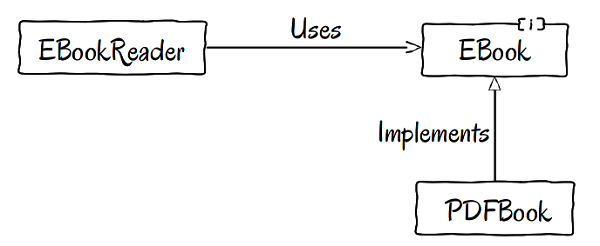
\includegraphics[scale=.4]{img/ebookreader-ebookinterface-pdfbook.png}
    \end{figure}
    \begin{exampleblock}{Good}
        \begin{itemize}
            \item Jetzt hängt \texttt{EBookReader} nur noch von einem abstrakten Interface (\texttt{EBook}) ab.
            \item \texttt{PDFBook} kann nun dieses Interface implementieren und ein \texttt{EBookReader} kann somit auch ein \texttt{PDFBook} lesen.
        \end{itemize}
    \end{exampleblock}

    \vspace{.1in}
    \footnotesize
    \url{http://code.tutsplus.com/series/the-solid-principles}
    \vspace{.1in}
\end{frame}

\begin{frame}{\quad}
    \center
    \Huge{\textbf{5}}
\end{frame}

\begin{frame}{Tipp 5}
    \begin{block}{}
        \center
        \textsc{\quotes{Draw diagrams.}}
    \end{block}
\end{frame}

\begin{frame}{Tipp 5: Draw diagrams.}
    \begin{itemize}
        \item Diagramme können hilfreich sein, ein Problem besser zu erfassen.
        \item Beispiele
        \begin{itemize}
            \item Zusammehänge zwischen verschiedenen Objekten
            \item Flussdiagramme
            \item Abhängigkeiten zwischen Klassen
            \item Skizze bei geometrischen Problemen
            \item Graphen
        \end{itemize}
        \item Das Diagramm muss nicht perfekt sein.
    \end{itemize}
\end{frame}

\begin{frame}{\quad}
    \center
    \Huge{\textbf{6}}
\end{frame}

\begin{frame}{Tipp 6}
    \begin{block}{}
        \center
        \textsc{\quotes{Do not query.}}
    \end{block}
\end{frame}

\begin{frame}{Tipp 6: Do not query.}
    \begin{itemize}
        \item Objekte sollten sich ihrem Zustand entsprechend \textbf{verhalten}.
        \item Objekte sollten \textit{nicht} ihrem Zustand entsprechend \textbf{verwendet werden}.
    \end{itemize}
\end{frame}

\begin{frame}[fragile]{Tipp 6: Do not query.}
    \begin{alertblock}{Bad}
        \begin{lstlisting}[language=Java,basicstyle=\scriptsize]
class Article {
    private int stock;

    public int getStock() {
        return this.stock;
    }

    public void sell(int quantity) {
        this.stock -= quantity;
    }
}

if (article.getStock() >= quantity) {
    article.sell(quantity);
} else {
    System.out.println("This article is currently unavailable.");
}
        \end{lstlisting}
    \end{alertblock}
\end{frame}

\begin{frame}[fragile]{Tipp 6: Do not query.}
    \begin{alertblock}{Still bad}
        \begin{lstlisting}[language=Java,basicstyle=\scriptsize]
class Article {
    private int stock;

    public void sell(int quantity) {
        if (this.stock >= quantity) {
            this.stock -= quantity;
        } else {
            System.out.println("This article is currently unavailable.");
        }
    }
}

article.sell(quantity);
        \end{lstlisting}
    \end{alertblock}
\end{frame}

\begin{frame}[fragile]{Tipp 6: Do not query.}
    \begin{exampleblock}{Good}
        \begin{lstlisting}[language=Java,basicstyle=\scriptsize]
class Article {
    private int stock;

    public boolean sell(int quantity) {
        if (this.stock >= quantity) {
            this.stock -= quantity;
            return true;
        }
        return false;
    }
}

if (!article.sell(quantity)) {
    System.out.println("This article is currently unavailable.");
}
        \end{lstlisting}
    \end{exampleblock}
\end{frame}

\begin{frame}[fragile]{Tipp 6: Do not query.}
    \begin{block}{Even better}
        \begin{lstlisting}[language=Java,basicstyle=\scriptsize]
class Article {
    private int stock;

    public boolean sell(int quantity) {
        if (quantity <= 0) {
            throw new IllegalArgumentException(
                "Negative or null quantity was given.");
        }
        if (quantity > this.stock) {
            return false;
        }
        this.stock -= quantity;
        return true;
    }
}

if (!article.sell(quantity)) {
    System.out.println("This article is currently unavailable.");
}
        \end{lstlisting}
    \end{block}
\end{frame}

\begin{frame}{\quad}
    \center
    \Huge{\textbf{7}}
\end{frame}

\begin{frame}{Tipp 7}
    \begin{block}{}
        \center
        \textsc{\quotes{Avoid floating point numbers if possible.}}
    \end{block}
\end{frame}

\begin{frame}{Tipp 7: Avoid floats.}
    \begin{itemize}
        \item Man sollte sich immer genau überlegen, ob man Gleitkommazahlen verwenden möchte.
        \item Gleitkommazahlen können u. U. tü­ckisch sein. (vgl. Genauigkeit, Epsilon-Vergleich)
        \item Gleitkommazahlen sind auch sehr viel rechenaufwendiger als ganze Zahlen.
        \item Ein paar Beispiele:
        \begin{itemize}
            \item Man kann \euro 1.99 auch einfach als Ganzzahl (199) darstellen.
            \item Das Vergleichen von Abständen zwischen Punkten geht auch ohne die euklidische Norm
            $\sqrt{(x_0 - x_1)^2 + (y_0 - y_1)^2}$ mit samt der Wurzel als Gleitkommazahl zu berechnen.\\
            Es genügt, wenn man $(x_0 - x_1)^2 + (y_0 - y_1)^2$ berechnet.\\
            Bei ganzzahligen Koordinaten ist das Ergebnis wieder eine ganze Zahl.
        \end{itemize}
    \end{itemize}
\end{frame}

\begin{frame}{\quad}
    \center
    \Huge{\textbf{8}}
\end{frame}

\begin{frame}{Tipp 8}
    \begin{block}{}
        \center
        \textsc{Datenkapselung}
    \end{block}
\end{frame}

\begin{frame}{Tipp 8: Datenkapselung}
    \begin{itemize}
        \item Attribute sollten \textbf{immer} \texttt{private} (manchmal \texttt{protected}) sein.
        \item Getter und Setter (nur wenn sinnvoll) verwenden.
        \item Im Setter kann überprüft werden, ob übergebene Werte sinnvoll sind.
        \item Nur die Methoden auf \texttt{public} setzen, welche auch von außen sichtbar sein müssen.
        \item So wenig wie möglich (am besten garnichts) über Implementierungsdetails preisgeben.
        \item Beim Entwurf einer Klasse, auch die Perspektive von Client-Klassen berücksichtigen und sich die Fragen stellen:\\
        \begin{itemize}
            \item Was muss ich wissen, um diese Klasse sinnvoll zu verwenden ?
            \item Welche Methoden/Schnittstelle benötige ich ?
            \item Gibt es evtl. unnötige Details, die nach außen sichtbar sind ?
        \end{itemize}

    \end{itemize}
\end{frame}

\begin{frame}{\quad}
    \center
    \Huge{\textbf{9}}
\end{frame}

\begin{frame}{Tipp 9}
    \begin{block}{}
        \center
        \textsc{Unterscheide zwischen\\ \textbf{Datenstrukturen} und \textbf{abstrakten Datentypen}.}
    \end{block}
\end{frame}

\begin{frame}{Tipp 9: Datenstruktur vs. abstrakter Datentyp}
    \begin{itemize}
        \item Eine \textbf{Datenstruktur} ist eine konkrete Anordnung/Organisation/Speicherung von Daten im Rechner.
        \vspace{.2in}
        \item \textbf{Abstrakte Datentypen} hingegen verraten nichts über eine mögliche Implementierung.
    \end{itemize}
\end{frame}

\begin{frame}{Tipp 9: Datenstruktur vs. abstrakter Datentyp}
    Quiz: \textbf{Datenstruktur} oder \textbf{abstrakter Datentyp}
    \begin{itemize}
        \item Queue
        \item Stack
        \item Heap
        \item Map
        \item PriorityQueue
        \item HashMap
        \item Array
        \item Graph
    \end{itemize}
\end{frame}

\begin{frame}{Tipp 9: Datenstruktur vs. abstrakter Datentyp}
    Lösung:
    \begin{itemize}
        \item Queue: \alert{abstrakter Datentyp}
        \item Stack: \alert{abstrakter Datentyp}
        \item Heap: \alert{Datenstruktur}
        \item Map: \alert{abstrakter Datentyp}
        \item Priority Queue: \alert{abstrakter Datentyp}
        \item Hash Map: \alert{Datenstruktur}
        \item Array: \alert{Datenstruktur}
        \item Graph: \alert{abstrakter Datentyp}
    \end{itemize}
\end{frame}

\begin{frame}{\quad}
    \center
    \Huge{\textbf{10}}
\end{frame}

\begin{frame}{Tipp 10}
    \begin{block}{}
        \center
        \textsc{Verwende aussagekräftige Bezeichner.}
    \end{block}
\end{frame}

\begin{frame}{\quad}
    \center
    \Huge{\textbf{11}}
\end{frame}

\begin{frame}{Tipp 11}
    \begin{block}{}
        \center
        \textsc{\quotes{Exceptions sind Ausnahmesituationen, nicht Kontrollfluss.}}
    \end{block}
\end{frame}

\begin{frame}{\quad}
    \center
    \Huge{\textbf{12}}
\end{frame}

\begin{frame}{Tipp 12}
    \begin{block}{}
        \center
        \textsc{\quotes{Comment your code.}}
    \end{block}
\end{frame}

\begin{frame}{Tipp 12: Comment your code.}
    \begin{itemize}
        \item Kommentare beschreiben \textbf{Logik}, nicht Java-Syntax.
        \item Javadoc verwenden !
        \begin{itemize}
            \item Kurz die Aufgabe der Klasse/Methode beschreiben.
            \item Parameter (Typ und Semantik) (\texttt{@param})
            \item Rückgabewert (Typ und Semantik) (\texttt{@return})
            \item Exceptions ? (\texttt{@throws})
        \end{itemize}
    \end{itemize}
\end{frame}

\begin{frame}[fragile]{Tipp 12: Comment your code.}
    \begin{itemize}
        \item Kommentare beschreiben Logik, nicht Java-Syntax.
    \end{itemize}
    \begin{columns}[c]
        \column{.5\textwidth}
        \begin{alertblock}{Not so good}
            \begin{lstlisting}[language=Java,basicstyle=\scriptsize]
// check if a bigger than b
if (a > b) {
    // check if a bigger than c
    if (a > c) {
        // returns a
        return a;
    }
    // returns c
    return c;
// check if b bigger than c
} else if (b > c) {
    // returns b
    return b;
}
// returns c
return c;
            \end{lstlisting}
        \end{alertblock}
        \column{.5\textwidth}
        \begin{exampleblock}{Better}
            \begin{lstlisting}[language=Java,basicstyle=\scriptsize]
// return the maximum of a, b, and c
if (a > b) {
    if (a > c) {
        return a;
    }
    return c;
} else if (b > c) {
    return b;
}
return c;
            \end{lstlisting}
        \end{exampleblock}
    \end{columns}
\end{frame}

\begin{frame}[fragile]{Tipp 12: Comment your code.}
    \begin{itemize}
        \item Javadoc verwenden !
    \end{itemize}
    \begin{exampleblock}{Klasse}
        \begin{lstlisting}[language=Java,basicstyle=\tiny]
/**
 * Recursive descent parser for the recommend command.
 *
 * @version 1.1
 * @author YouniS Bensalah <younis.bensalah@riseup.net>
 */
class RecommendParser { ... }
        \end{lstlisting}
    \end{exampleblock}
\end{frame}

\begin{frame}[fragile]{Tipp 12: Comment your code.}
    \begin{itemize}
        \item Javadoc verwenden !
    \end{itemize}
    \begin{exampleblock}{Methode}
        \begin{lstlisting}[language=Java,basicstyle=\tiny]
/**
 * Parse the term and return its meaning, i.e., a set of Products.
 *
 * @param code The line containing the term.
 * @return The set of recommended Products.
 * @throws SyntaxException if the term did not match the specified syntax rules.
 * @throws InvalidNodeException if the required node does not exist.
 */
public Set<Product> parse(String code) throws SyntaxException, InvalidNodeException { ... }
        \end{lstlisting}
    \end{exampleblock}
\end{frame}

\begin{frame}{Tipp 12: Comment your code.}
    \begin{itemize}
        \item \textbf{How to Write Doc Comments for the Javadoc Tool}\\
        \url{http://www.oracle.com/technetwork/articles/java/index-137868.html}
    \end{itemize}
\end{frame}

\begin{frame}{\quad}
    \center
    \Huge{\textbf{13}}
\end{frame}

\begin{frame}{Tipp 13}
    \begin{block}{}
        \center
        \textsc{\quotes{Avoid Tour-de-France code.}}
    \end{block}
\end{frame}

\begin{frame}{Tipp 13: Avoid Tour-de-France code.}
    \begin{columns}[c]
        \column{.5\textwidth}
        \begin{block}{}
            \center
            \textsc{\quotes{Avoid Tour-de-France code.}}
        \end{block}
        \begin{itemize}
            \item Langen, unübersichtlichen Code in sinnvolle Methoden aufteilen.
            \item Max. 30 Zeilen in einer Methode.
            \item Tiefe Verschachtelung vermeiden !
        \end{itemize}
        \column{.5\textwidth}
        \begin{figure}
            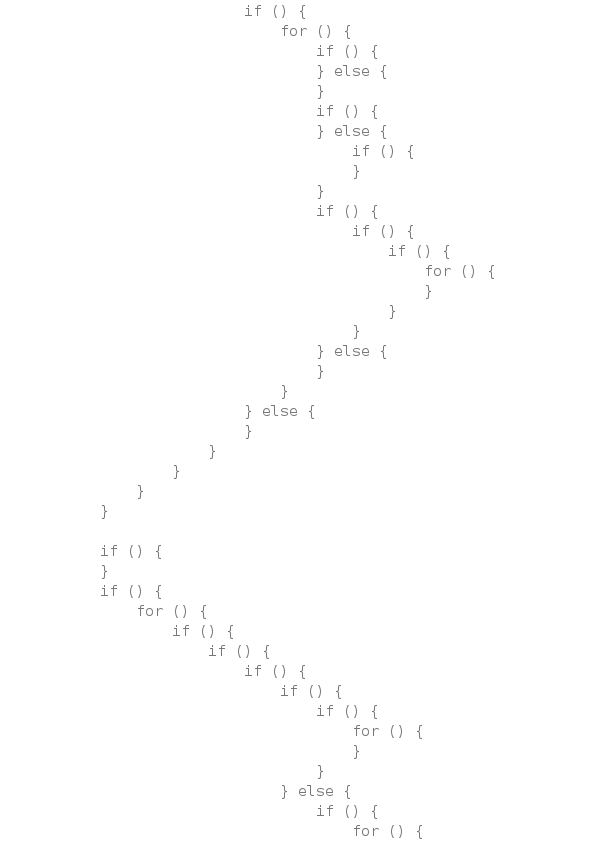
\includegraphics[scale=.3]{img/tourdefrancecode1.png}
        \end{figure}
    \end{columns}
\end{frame}

\begin{frame}{Tipp 13: Avoid Tour-de-France code.}
    \begin{itemize}
        \item \textit{Tour-de-France code}
    \end{itemize}

    \begin{figure}
        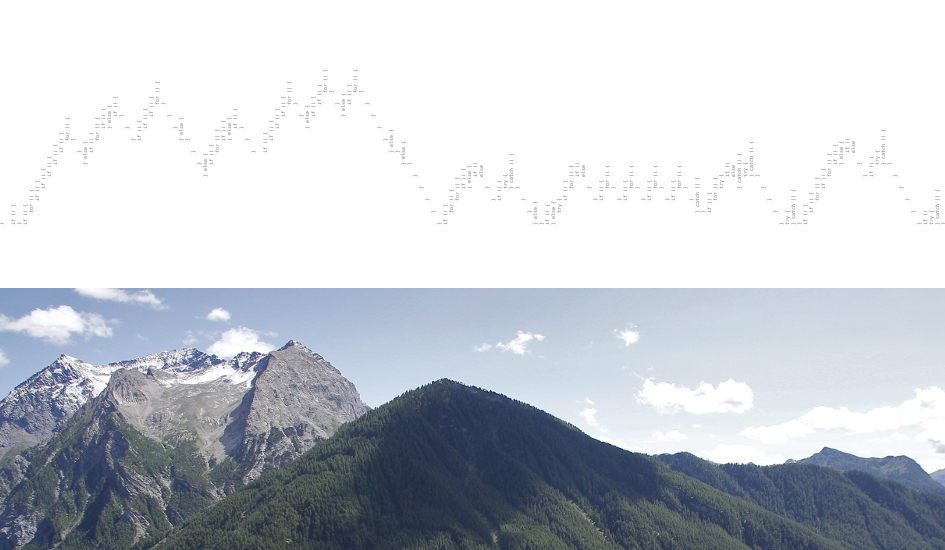
\includegraphics[scale=.4]{img/tourdefrancecode2.png}
    \end{figure}
\end{frame}

\begin{frame}{\quad}
    \center
    \Huge{\textbf{14}}
\end{frame}

\begin{frame}{Tipp 14}
    \begin{block}{}
        \center
        \textsc{\quotes{Use enums.}}
    \end{block}
\end{frame}

\begin{frame}{Tipp 14: Use enums.}
    \begin{itemize}
        \item \texttt{if (today == Day.FRIDAY)} ist lesbarer als \texttt{if (today == 5)}.
        \item Es schleichen sich nicht so leicht Fehler ein.
        \begin{itemize}
            \item Ist \quotes{Montag} oder \quotes{Sonntag} der erste Tag der Woche ?
            \item Fängt man hier bei 0 oder bei 1 an zu zählen ?
            \item Welche Werte sind nochmal gültig ?
        \end{itemize}
    \end{itemize}
\end{frame}

\begin{frame}{\quad}
    \center
    \Huge{\textbf{15}}
\end{frame}

\begin{frame}{Tipp 15}
    \begin{block}{}
        \center
        \textsc{\quotes{Auf sauber formatierten Code achten (i.e., Checkstyle)}}
    \end{block}
\end{frame}

\begin{frame}{\quad}
    \center
    \Huge{\textbf{16}}
\end{frame}

\begin{frame}{Tipp 16}
    \begin{block}{}
        \center
        \textsc{\quotes{Always test your code.}}
    \end{block}
\end{frame}

\section{Debugging}

\begin{frame}{\quad}
    \center
    \Huge{\dots und dann noch Debugging}
\end{frame}

\begin{frame}{Wiederholung: Debugging}
    \textbf{Debugging}: Finden und Entfernen von Fehlern (Bugs) in einem Programm

    Praktische Tipps:
    \begin{itemize}
        \item Code erneut durchlesen
        \item Verschiedene Eingaben testen und genau auf Resultat achten
        \item Inhalte an verschiedenen Stellen im Programm ausgeben lassen
        \item An geeigneten Stellen feste Werte reinschreiben und schauen was dann passiert
        \item Debugger verwenden
        \item \textbf{Breakpoints setzen !}
        \item \dots
    \end{itemize}
\end{frame}

\begin{frame}{Debugging: Breakpoints}
    \begin{itemize}
        \item \textbf{Breakpoints} (Haltepunkte) erleichtern das finden von Fehlerursachen im Quellcode.
        \item Idee: Programm \quotes{in Zeitlupe} laufen lassen.
        \item Vorgehensweise:
        \begin{enumerate}
            \item Setze \textbf{Breakpoint} an \quotes{kritische} Stelle im Code.
            \item Führe das Programm im \textbf{Debug-Modus} aus.
            \item Das Programm wird an der markierten Stelle \alert{halten}.
            \item Der Programmierer hat die Chance, den Zustand es Programms zu untersuchen und nach Anomalien zu suchen (z. B. den Inhalt von Variablen anschauen).
        \end{enumerate}
        \item Alle gängigen IDEs (Eclipse, NetBeans, \dots) unterstützen das Setzen von Breakpoints.
    \end{itemize}
\end{frame}

\appendix
\beginbackup

\begin{frame}{Wiederholung: Graphen}
    \begin{figure}
        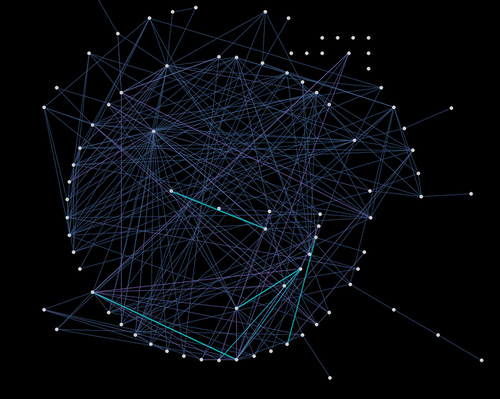
\includegraphics[scale=.4]{img/graph_4fj49f4.jpg}
    \end{figure}
\end{frame}

\begin{frame}{Wiederholung: Graphen}
        \begin{block}{Definition}
            Ein \textbf{Graph} ist ein Paar $\mathcal{G} = (\mathcal{V}, \mathcal{E})$
            mit $\mathcal{V}$ Menge von Knoten
            und $\mathcal{E} \subset \mathcal{V} \times \mathcal{V}$ Menge von Kanten.
        \end{block}
        \begin{exampleblock}{}
            \begin{itemize}
                \item $\mathcal{V} = \left\{ A, B, C, D, E, F \right\}$
                \item $\mathcal{E} = \left\{ (A, B), (B, C), (C, E), (D, B), (E, D), (E, F) \right\}$
            \end{itemize}
        \end{exampleblock}
        \begin{figure}
            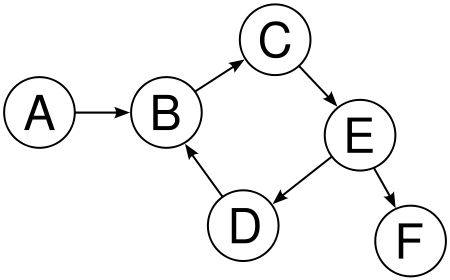
\includegraphics[scale=.3]{img/graph.png}
        \end{figure}
\end{frame}

\begin{frame}{Wiederholung: Adjazenzmatrix}
    \[
    \left(
    \begin{array}{cccccc}
        0 & 1 & 0 & 0 & 0 & 0 \\
        0 & 0 & 1 & 0 & 0 & 0 \\
        0 & 0 & 0 & 0 & 1 & 0 \\
        0 & 1 & 0 & 0 & 0 & 0 \\
        0 & 0 & 0 & 1 & 0 & 1 \\
        0 & 0 & 0 & 0 & 0 & 0
    \end{array}
    \right)
    \]
    \begin{figure}
        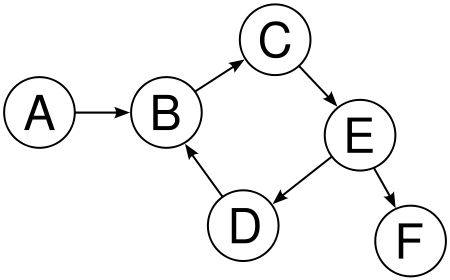
\includegraphics[scale=.3]{img/graph.png}
    \end{figure}
\end{frame}

\begin{frame}{Wiederholung: Adjazenzmatrix}
    \[
    \left(
    \begin{array}{cccccc}
        0 & 1 & 0 & 0 & 0 & 0 \\
        0 & 0 & 1 & 0 & 0 & 0 \\
        0 & 0 & 0 & 0 & 1 & 0 \\
        0 & 1 & 0 & 0 & 0 & 0 \\
        0 & 0 & 0 & 1 & 0 & 1 \\
        0 & 0 & 0 & 0 & 0 & 0
    \end{array}
    \right)
    \]
    \begin{itemize}
        \item Adjazenzmatrix speichert, welche Knoten des Graphen durch eine Kante verbunden sind
        \item Zeilen entsprechen den Startknoten, Spalten entsprechen den Zielknoten
        \item $1$ bedeutet, dass eine Kante existiert, $0$ bedeutet, dass die Knoten \textit{nicht} verbunden sind
    \end{itemize}
\end{frame}

\begin{frame}{Fragen ?}
    \begin{figure}
        
\includegraphics[scale=.3]{img/Question-Rage-Face.jpg}
    \end{figure}
\end{frame}

\begin{frame}{Bis nächste Woche !}
    \begin{figure}
        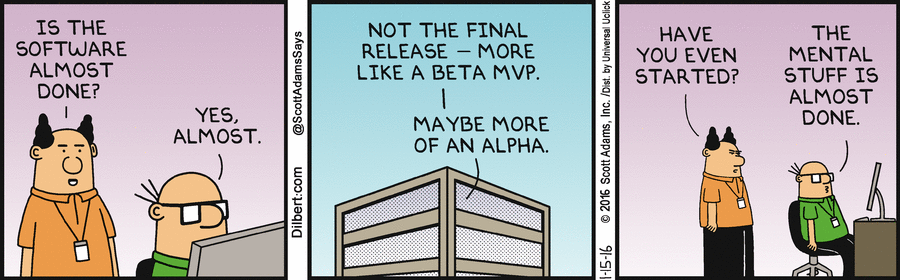
\includegraphics[scale=.4]{img/dt160115.png}
    \end{figure}
\end{frame}

\backupend

\end{document}
